\chapter{Preliminary Work}\label{chap:chap3}

In the initial step of work, we superficially explored ChatGPT's ability to generate tests for an example conflict of Point, where a distance method is altered from euclidean to manhattan in one branch and in the other branch, a move method is changed from using the value 1 for x and y movement to using the result of the distance calculation.

We tested two frameworks, first just asking for a test, with prompts based on the testing indications given by the DSL for the case:

\begin{itemize}
  \item A Dependency Based semantic conflict was possibly introduced in a 3-way merge. Develop a test for the class Point, that covers the methods move() and distance(), without calling distance() directly.
Before the merge, the class under test was: [base Point]
After the merge, it was: [merged Point].
  \item A Dependency Based semantic conflict was possibly introduced in a 3-way merge. Develop a test for the class Point, that covers the methods move() and distance(), without calling distance() directly.
Before the merge, the class under test was: [base Point]
In the branch A it was changed to: [A Point]
In the branch B it was changed to: [B Point]
After the merge, it was: [merged Point].

\end{itemize}

For this, the LLM simply took one version and created tests taking it as correct behaviour. In the first case, for Base and in the second for Merge. This is not ideal, as the first does not allow us to distinguish if the behaviour changed due to merging, or just do to changes in the branches. The latter takes merge as correct behaviour and will thus always fail.

Other tests involved first asking for an explanation if there was a merge conflict there, before asking for a test

\begin{itemize}
  \item We have done a merge on a piece of code code.
Before the merge, the code was: [code]
In the branch A it was changed to: [code]
In the branch B it was changed to: [code]
After the merge it was: [code]
Do you believe there could be a merge conflict here? Where? Explain why.
  \item We have done a merge on a piece of code code.
Before the merge, the code was: [code]
In the branch A it was changed to: [code]
In the branch B it was changed to: [code]
After the merge it was: [code]
Do you believe there could be a merge conflict here? Where? Explain why. Pay attention to both additions and modifications.
  \item We have done a merge on a piece of code code.
Before the merge, the code was: [code]
In the branch A it was changed to: [code]
In the branch B it was changed to: [code]
After the merge it was: [code]
Do you believe there could be a *semantic* merge conflict here? Where? Explain why. Pay attention to both additions and modifications.

\end{itemize}

The first two prompts failed. Indeed for prompt ChatGPT only mentioned the changes in move, but even after prompting it to pay attention to distance, it failed to identify the conflict. For both, it seemed to not understand what was being referred to when speaking of conflict, describing all changes as a "conflict". Thus it would say, there is a conflict between whether to use euclidian and manhattan distance and there is a conflict on how the move function works.

The last prompt given, highlighting the *semantic* aspect of the merge conflict, yielded good results, with the conflict being perfectly described. After prompting for a test, it generates an appropriate one: it tests if the move function updates Point appropriately based on the euclidean distance. Thus it fails for base and branch B, where movement is still done with the value of 1, it passes for branch A as there move is based on distance; and it fails in merge, as now movement is being done with the distance calculation, but the calculation is now manhattan.

\begin{figure}
    \centering
    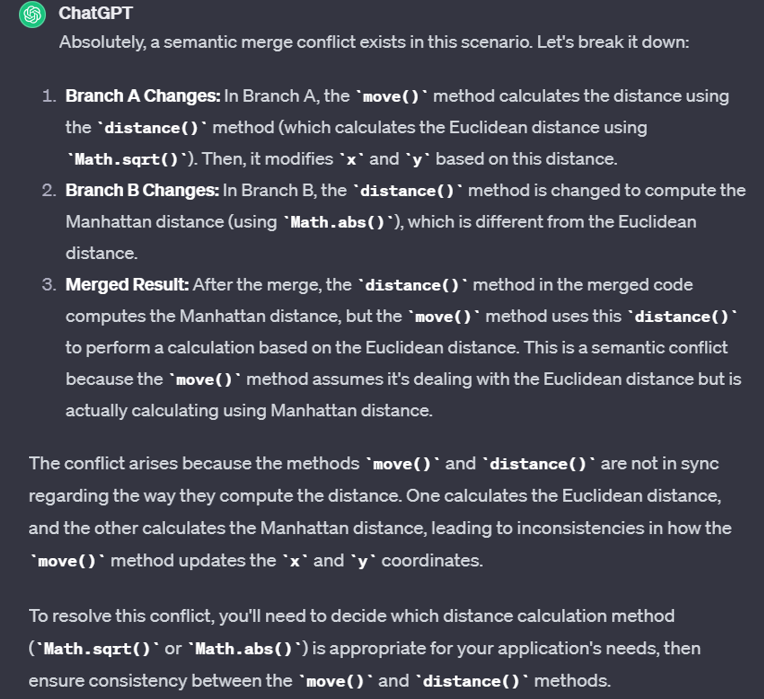
\includegraphics[width=0.75\linewidth]{figures/image.png}
    \caption{ChatGPT description of the semantic conflict}
    \label{fig:enter-label}
\end{figure}



In the future we will also look at other LLMs, specifically Llama.